\documentclass[UTF8]{ctexart}
\usepackage{mathtools,amsmath,graphicx,array,verbatim,booktabs}
%verbatim是注释宏包
\usepackage{float}

\begin{document}
	
	%标题设置:
    \title{\textbf{我要笑遍全世界的\LaTeX 基础笔记}}%\Latex是专属标记专业一点
    \author{wyxbqsj}
    \date{2020-7-6} %date命令删去会自动生成日期,但格式为:2020年7月6日;不想要出现日期的话,就用\date{},花括号内为空,日期就不会显示了
    \maketitle %未加该命令前,标题、作者等样式不显示
    
    %章节设置:
    \section{LaTex的使用}
    \subsection{LaTex的基础知识}
    \subsubsection{LaTex的结构}
    LaTex我们一般分为以下三个部分:
    
    \begin{enumerate}
    	\item 说明文档类型( 我想写一篇文章)
    	\item 说明用的宏包(我要写一篇文章)
    	\item 文档环境(我正在写一篇文章)
    \end{enumerate}

    \subsubsection{LaTex 文档类型}
    有三个文档类型:文章(article)、报告(report)、书(book),中文的文章是ctexart,中文字体是UTF8
    
    代码就是:documentclass[UTF8]\{ctexart\} %{}前加\才能显示该符号
    
    \subsection{文章的写作}
    \begin{comment}
    1.中间空行才是换段
    
    2.加粗:\textbf{加粗命令}
    
    3.字体:\textbf{\songti字体为宋体并加粗}
    
    4.字号:\normalsize{默认字号,比五号字稍小一些是10pt的}
    
    \large{字号大点}
    
    \LARGE{字号更大点}
    
    \huge{大号字}
    
    \Huge{超大号字}
    
    大括号{}起到划定范围的作用,不用大括号则表示该命令及以下内容全部遵循该命令
    
    \normalsize
    5.居中:默认是居左,环境的开始用begin说明,环境的结束用end来说明
    
    \begin{center}
    这是居中环境
    \end{center}
    \end{comment}
    \begin{enumerate}
    	\item 中间空行才是换段
    	
    	\item 加粗:textbf
    	
    	\item 字体:$\backslash$ textbf\{$\backslash$ songti字体为宋体并加粗\}
    	
    	\item 字号:$\backslash$normalsize,默认字号,比五号字稍小一些是10pt的
    	
    	$\backslash$large,字号大点
    	
    	$\backslash$LARGE,字号更大点
    	
    	$\backslash$huge,大号字
    	
    	$\backslash$Huge,超大号字,大括号\{\}起到划定范围的作用,不用大括号则表示该命令及以下内容全部遵循该命令
    	
    	\item 居中:默认是居左,环境的开始用begin说明,环境的结束用end来说明
    	
    	$\backslash$ begin\{center\}
    		这是居中环境
    	$\backslash$ end\{center\}
    \end{enumerate}
    \subsection{公式的写作}
    \subsubsection{行间公式:以下两个环境都可以让公式自动编号}
    \begin{comment}
    【 行间公式】
    	环境1:该环境内公式不可以换行
    	\begin{equation}
    	公式内容
    	\end{equation}
    	
    	环境2:该环境内公式可以换行,按如下方式换行
    	\begin{align}
    	&公式 \\  %&表示并列,\\表示换行
    	&公式
    	\end{align}
    【 行内公式】
        公式环境:$公式$
    \end{comment}
    \textbf{公式环境1:该环境内公式不可以换行}
    
    $\backslash$begin\{equation\}
    
    公式
    
    $\backslash$end\{equation\}
    
    \textbf{公式环境2:该环境内公式按如下方式换行}
    
    $\backslash$begin\{align\}
    
    \& 公式$\backslash$$\backslash$
    
    \&公式
    
    $\backslash$end\{align\}
    
    ~\\ %空行
    第一个公式:
    \begin{equation}
    	F=ma
    \end{equation}
    换行公式:
    \begin{align}
    	y&=ax^2 \notag \\ %notag命令使该行不编号
    	 &=bx^2  %按等号位置对齐
    \end{align}
    所有公式都不编号:
    \begin{equation*} %加星号*即可
    	y=ax
    \end{equation*}
    %简写方式:
    \[
        y=ax
    \]
    ~\\
    \subsubsection{行内公式}
    \textbf{公式环境:}\$公式\$
    
    例子,我们知道力与质量与加速度的关系为$F=ma$
    \subsubsection{一些公式命令}
    $x^{y}$ \qquad%幂
    $x_{y}$ \qquad%下标
    $\frac{x}{y}$ \qquad%分式
    $\sum_{n}^{i=1}$ \qquad%求和号
    $\int_{1}^{10}$ \qquad %积分号
    $\mathrm{x^2}$ \qquad%微分号
    
    \textbf{各种希腊字母:}
    
    $\alpha$ \qquad
    $\beta$ \qquad
    $\delta$ \qquad
    $\Delta$ \qquad
    $\gamma$ \qquad
    $\pi$ \qquad
    $\epsilon$ \qquad
    $\rho$ \qquad
    $\sigma$ \qquad
    $\sin{x}$ \qquad
    $\cos{x}$ \qquad
    $\tan{x}$ \qquad
    $\ln{x}$ \qquad
    $\sqrt{x}$ 
    
    \subsubsection{其他内容}
    \textbf{矩阵环境},需要提前加入宏包:mathtools
    	\begin{equation*}
    	A=\begin{bmatrix}
    	    1&2&3\\
    	    4&5&6\\
    	\end{bmatrix}
    	\end{equation*}
    \textbf{花括号},需要宏包mathtools
    \begin{equation*}
    	B=\begin{cases}
    	&x^2\\
    	&x^2+x\\
    	\end{cases}
    \end{equation*}
    
    \subsection{表格的输入}
    %\textbf{普通表格}环境使用tabular: 
    
    %\begin{tabular}{|l|c|r|} %l,c,r分别表示left,center,right,中间的竖线表示每一列加上竖线,少了哪个那一列就不加竖线
    %\hline %该行的行线
    %指标1&指标2&指标3\\ %每列之间用&隔开,每行之间用\\隔开
    %\hline
    %居左&居中&居右\\
    %\hline
    %\end{tabular}
    
    \textbf{三线表的制作}
    \begin{table}[!htbp] %h:放在此处 t:放在顶端 b:放在底端 p:在本页 如果是[htbp],意思就是优先放在此处,其次是每页的顶端,再次是底端
    	\centering
    	\caption{题目}
    	\begin{tabular}{cccc}
    		\toprule
    		&指标一&指标二&指标三\\
    		\midrule
    		方案一&1&2&3 \\
    		方案二&4&5&6 \\
    		\bottomrule
    	\end{tabular}
     \end{table}
 
 	\subsection{图片的插入}
 	用figure环境:
 	
 	\begin{figure}[hptb]
 		\centering
 		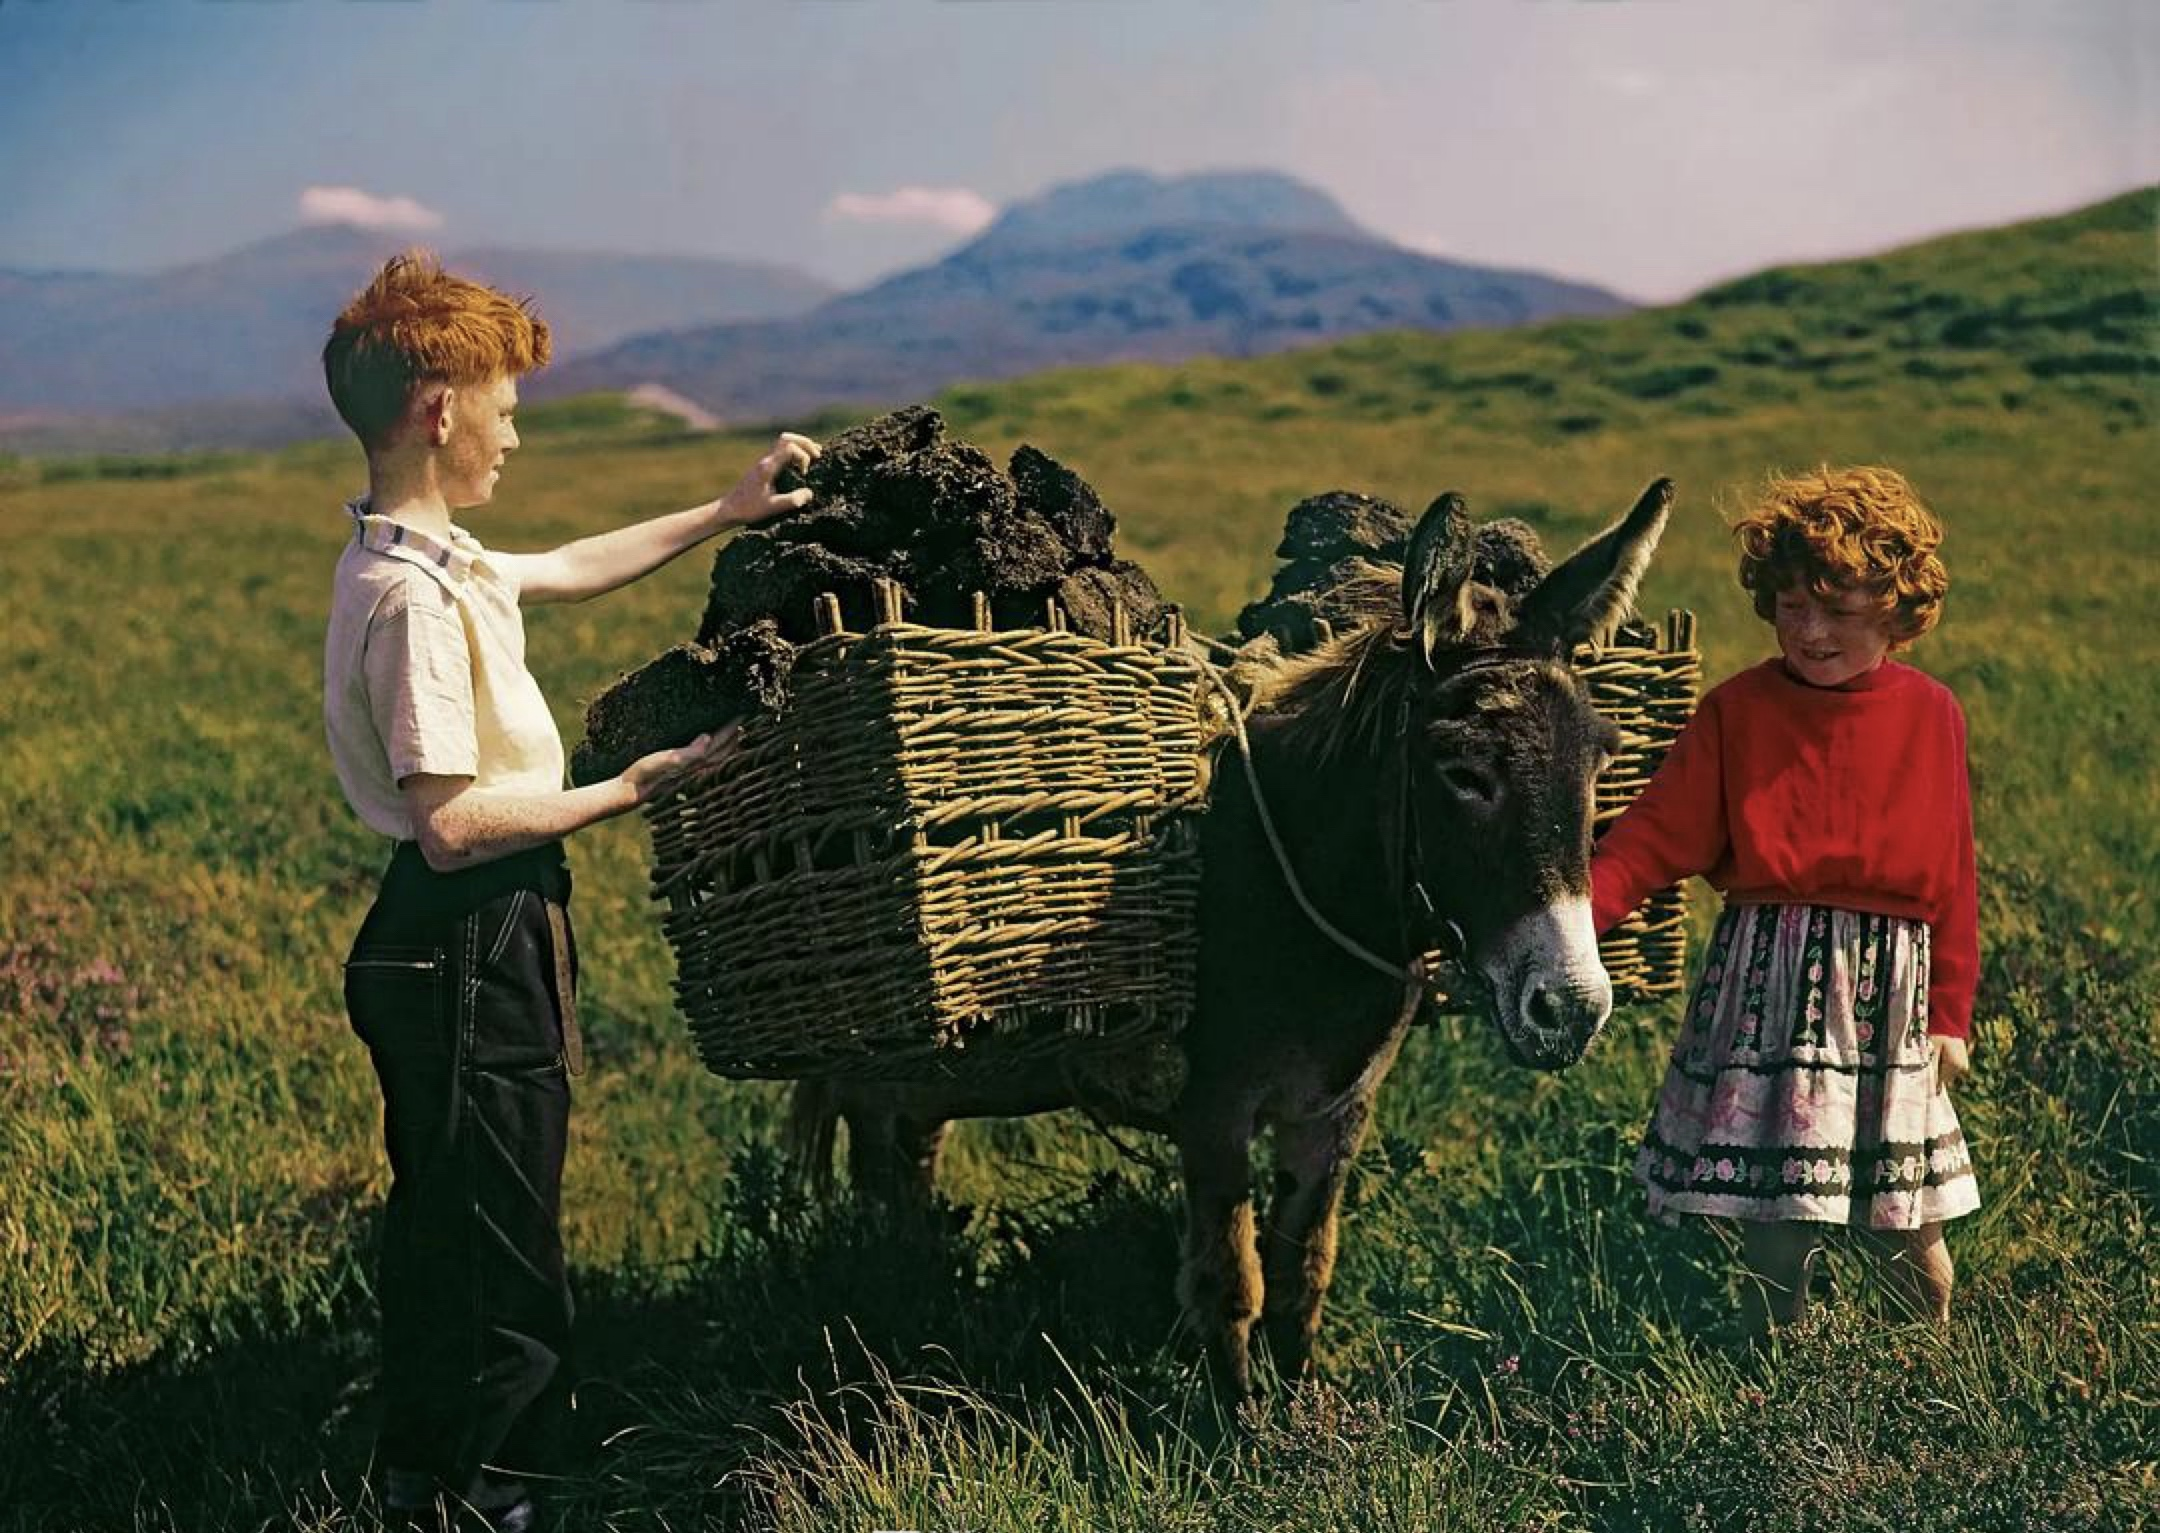
\includegraphics[width=0.7\linewidth]{name}
 		\caption{}
 		\label{fig:name}
 	\end{figure}
 
 	\subsection{命令lable的使用}
 	%\label{#1:#2} #1代表第一个参数,说明是什么类型的,有三种:eq公式,tab表格,fig图片;#2即为名字
 	label是标签,用来上下文中引用,相当于给加上标签的东西加了个名字,在上下文中只要用这个名字就知道是那个东西,如,将下面的公式命名为NiuDun:
 	\begin{equation}
 		F=ma \label{eq:NiuDun}
 	\end{equation}
 	现在来引用上面这个公式,请注意看(\ref{eq:NiuDun}),就会看到变化了。如此当公式很多时,前面插入一个公式(图片、表格等)编号都会自动编排,不需要再手动修改了!
 	
 	\section{LaTex的进阶}
 	\subsection{进阶公式}
 	\textbf{难点1:}解决不认识的符号:查资料或者百度
 	
 	\textbf{难点2:}放大版括号:放大版括号主要用来括住存在分式的式子,或者内部有很多括号的式子,用法是在左右括号分别加上$\backslash$left和$\backslash$right
 	\[
 		J_{r}=\dfrac{i\hbar}{2m}\left[\psi_{2}\dfrac{\partial\psi^*_2}{\partial_r}-\dots\right]
 	\]
 	
 	\textbf{难点3:}对齐多行等式:使用环境align来对齐多行等式,$\backslash$$\backslash$换行,\&对齐
 	\begin{align*}
 		(a+b)^{2}&=(a+b)(a+b) \\
 		         &=a^2+b^2+2ab
 	\end{align*}
 	
 	\textbf{难点4:}让公式的行号只出现在第二行,用$\backslash$notag命令
 	
 	~\\
 	现在我们完成那个复杂的公式:
 	\begin{align}
 		J_r&=\dfrac{i\hbar}{2m}\left[\psi_2\dfrac{\partial\psi^*_2}{\partial_r}-\psi^*\dfrac{\partial\psi_2}{\partial_r}\right] \notag \\
 		&=\dfrac{i\hbar}{2m}|f(\theta,\varphi)|^2\left[-\dfrac{ik}{r^2}-\dfrac{ik}{r^2}\right] \notag \\
 		&=\dfrac{v}{r^2}|f(\theta,\varphi)|^2
 	\end{align}
 	
    \subsection{进阶图片}
    主要是使用minipage环境对并排图片中的位置、标题的放置问题进行解决
    
    \textbf{minipage环境介绍:}minipage相当于可以将一个figure环境分成几个部分,minipage环境直接放在figure环境内就好
    
    \textbf{figure浮动环境中参数htbp介绍:}图片和表格在插入文章中会自己找相应的位置插入,不一定会出现在我们希望的位置上。为了限制他们这种浮动行为,我们就可以加上!htbp来禁止
    
    \textbf{标题caption的位置:}$\backslash$caption放置在哪里标题就会出现在哪里
    
    \textbf{minipage参数:} minipage环境后的必要参数用于界定两张并排图片占据当前行的宽度
    
    例图1:两张图片并排:行宽相加在1以内即可
     \begin{figure}[H]
    	\begin{minipage}{0.49\linewidth}
    		\centering
    		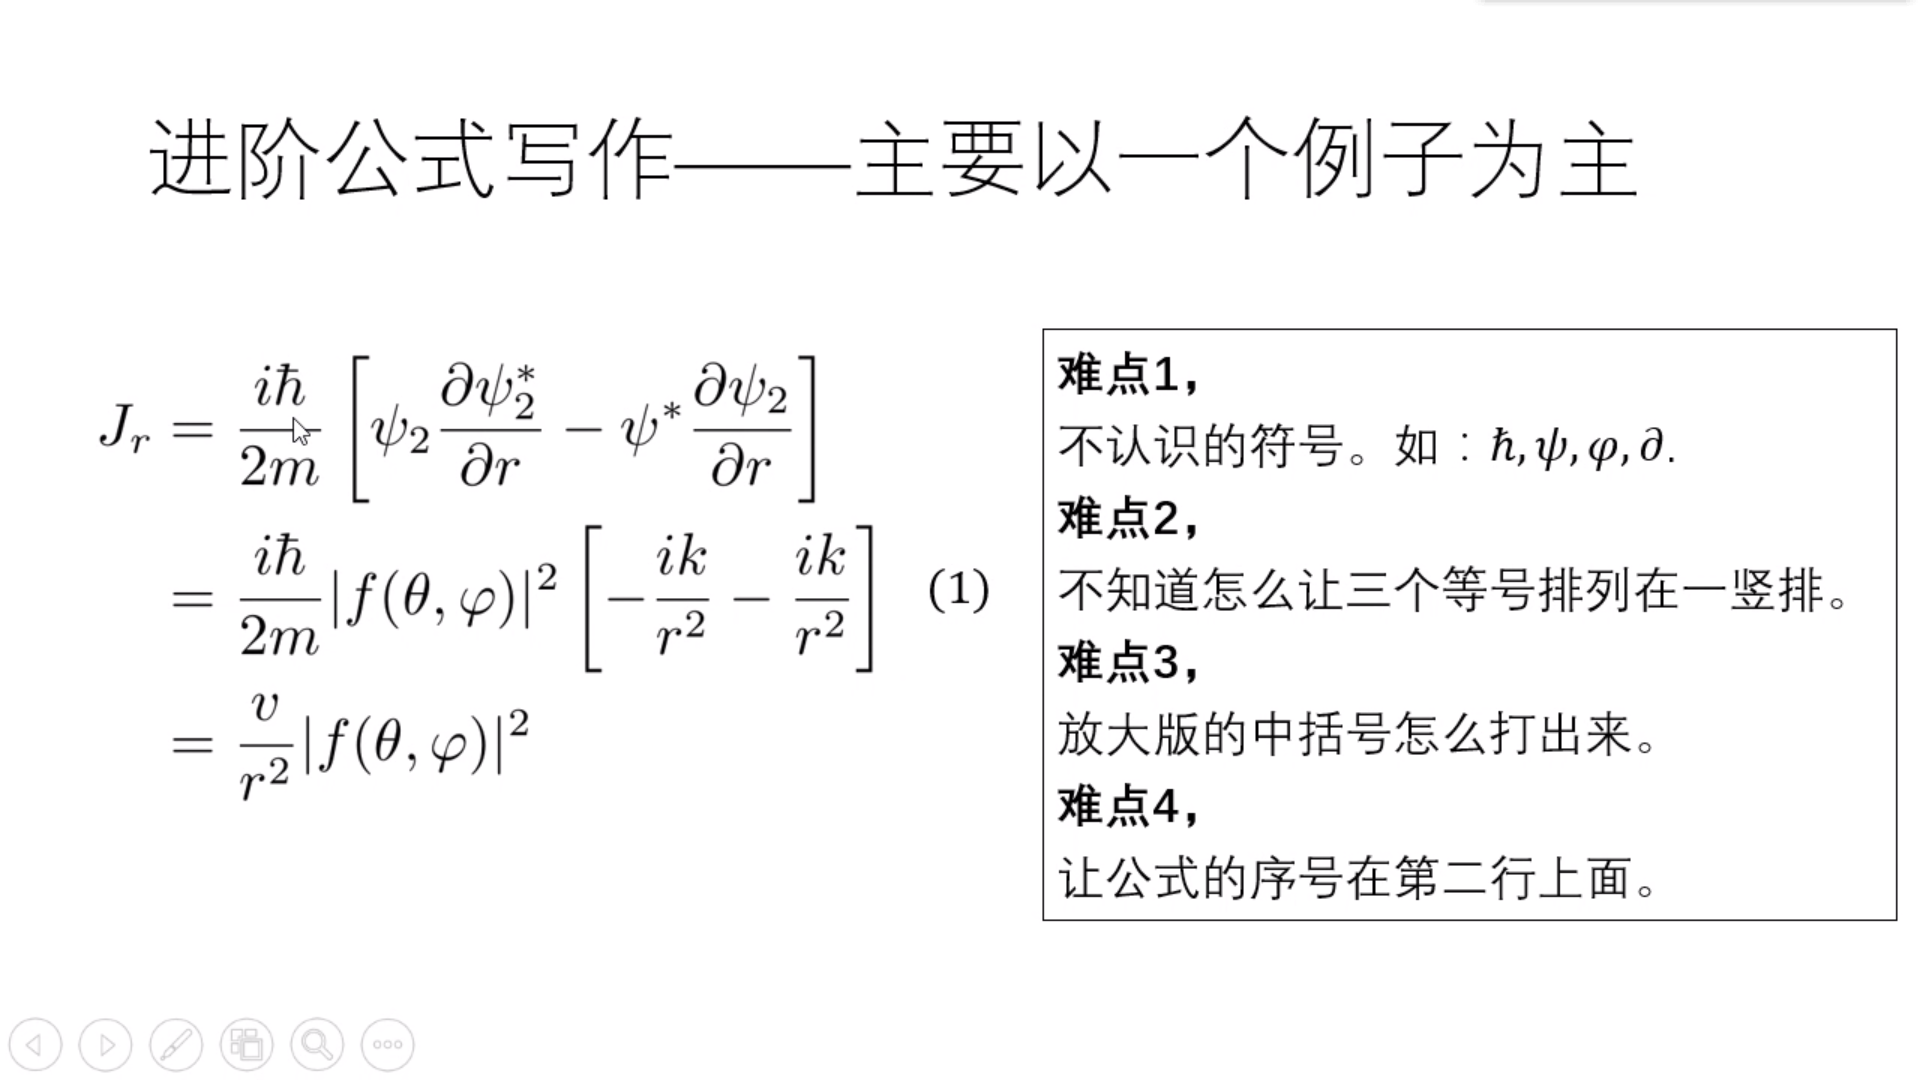
\includegraphics[width=4.0cm]{1.png}
    		\caption{左图的标题}
    	\end{minipage}
    	\begin{minipage}{0.49\linewidth}
    		\centering
    		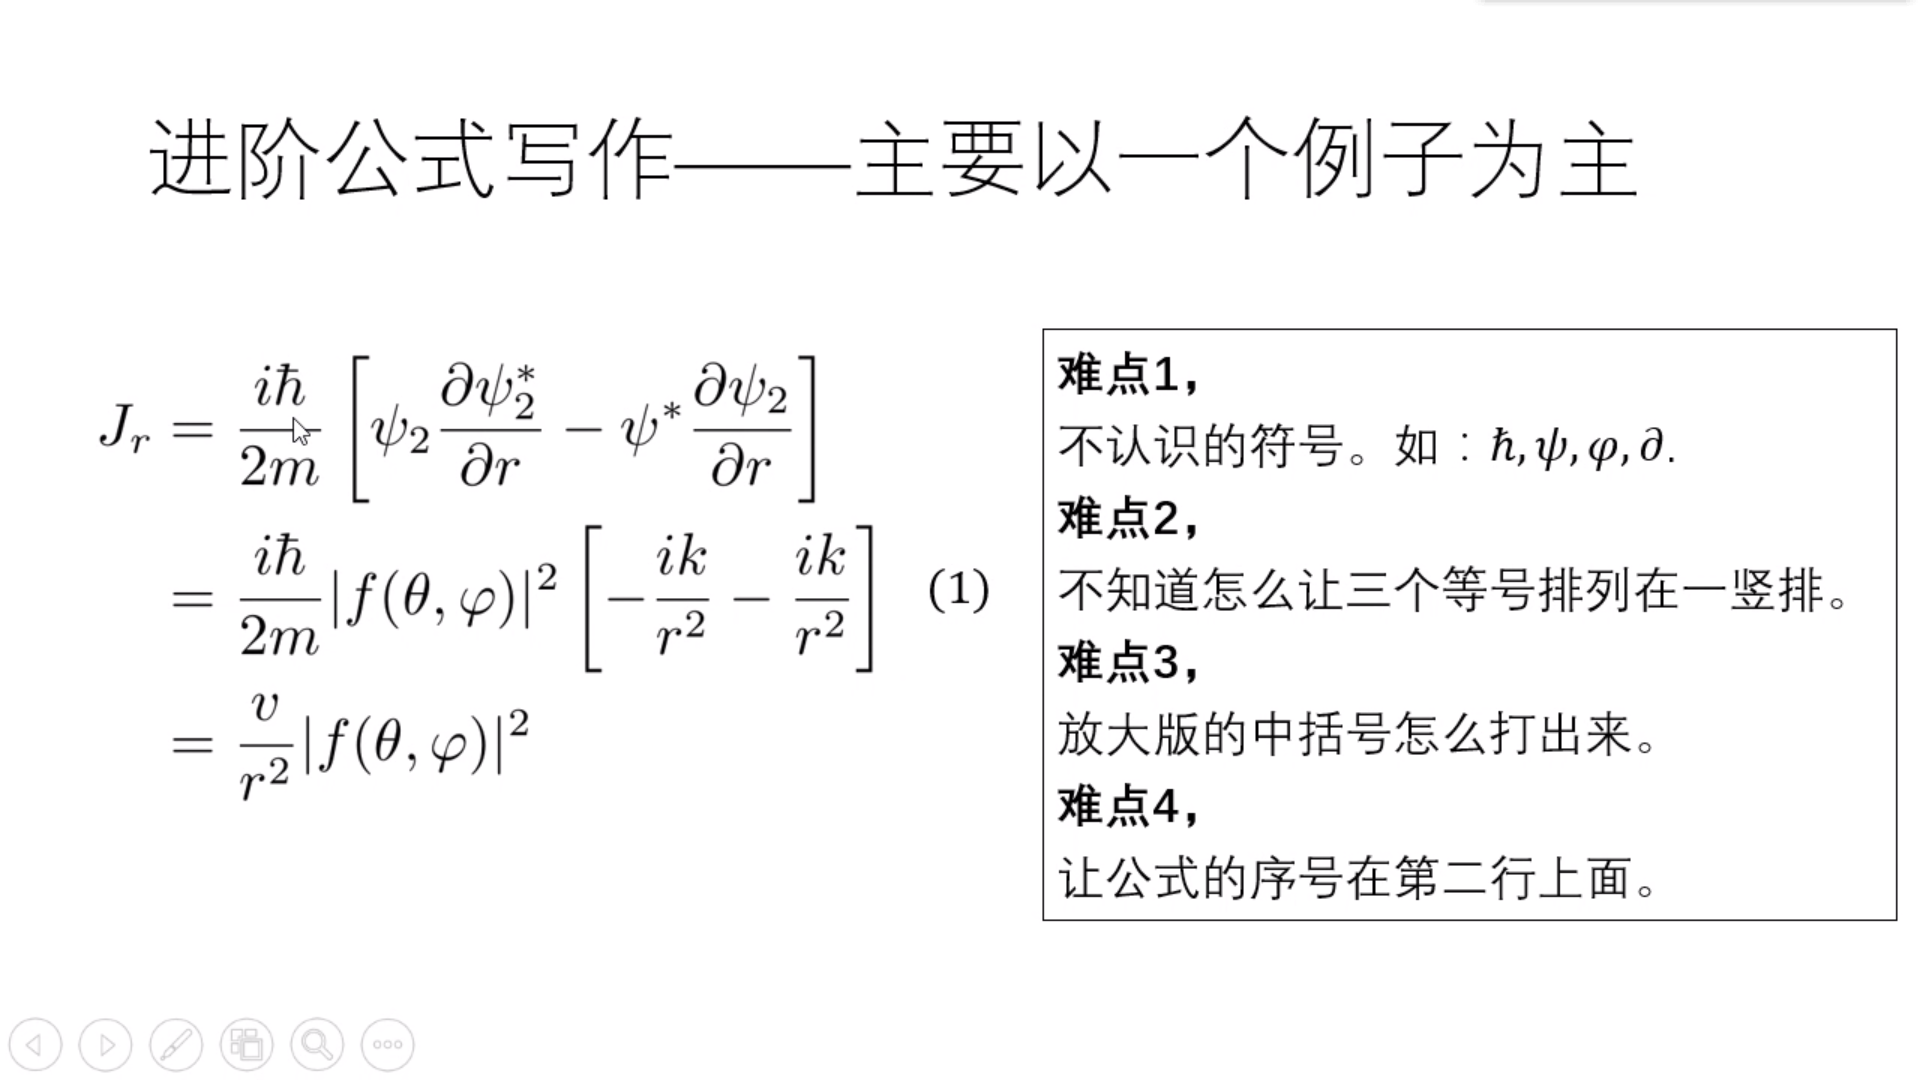
\includegraphics[width=4.0cm]{1.png}
    		\caption{右图的标题}
    	\end{minipage}
        \caption{最外面的标题}
    \end{figure}
    
    例图2:两张图片不并排
    \begin{figure}[!htbp]
    	\begin{minipage}{0.9\linewidth} %图片占行宽的9/10
    		\begin{flushright} %图片右端开始算
    			
\includegraphics[height=2cm]{2.jpg}
    			\caption{0.9行宽}
    		\end{flushright}
    	\end{minipage}
    	\begin{minipage}{0.5\linewidth} %图片占行宽的5/10
    		\begin{flushright} %图片右端开始算
    			
\includegraphics[height=2cm]{2.jpg}
    			\caption{0.5行宽}
    		\end{flushright}
    	\end{minipage}
    \end{figure}

    例图3:4张图片组合
    \begin{figure}
    	\begin{minipage}{0.5\linewidth}
    		\begin{flushright} %居右
    			
\includegraphics[height=2cm]{2.jpg}
    		\end{flushright}
    	\end{minipage}
    	\begin{minipage}{0.5\linewidth}
    		\begin{flushleft} %居左
    			
\includegraphics[height=2cm]{3.jpg}
    		\end{flushleft}
    	\end{minipage}
    	\begin{minipage}{0.5\linewidth}
    		\begin{flushright}
    			
\includegraphics[height=2cm]{2.jpg}
    		\end{flushright}
    	\end{minipage}
    	\begin{minipage}{0.5\linewidth}
    		\begin{flushleft}
    			
\includegraphics[height=2cm]{3.jpg}
    		\end{flushleft}
    	\end{minipage}
    	\caption{最大的标题}
    \end{figure}

	\subsection{进阶表格}
	表格线条粗细控制:$\backslash$toprule,$\backslash$midrule,$\backslash$bottomrule的可选参数,这三个指令需要用到booktabs包
		\begin{table}[H]
		\centering
		\caption{Definition and Varibles}
		\begin{tabular}{cll} 
			\toprule[0.2em]
			Symbol & Description & Value/Unit \\
			\midrule[0.12em]
			$m$ & 啦啦啦 & 嘎嘎嘎 \\
			$M$ & 啦啦啦 & 嘎嘎嘎 \\
			$R_e$ & 啦啦啦 & 嘎嘎嘎 \\
			\bottomrule[0.2em]
		\end{tabular}
	\end{table}
调整表格宽度:
	\begin{table}[H]
		\centering
		\caption{Definition and Varibles}
		\begin{tabular}{p{2cm}p{7cm}p{2cm}} %p表示要修改宽度,默认是居左,p后面的花括号内的数值表示该列的宽度
			\toprule[0.2em]
			Symbol & Description & Value/Unit \\
			\midrule[0.12em]
			$m$ & 啦啦啦 & 嘎嘎嘎 \\
			$M$ & 啦啦啦 & 嘎嘎嘎 \\
			$R_e$ & 啦啦啦 & 嘎嘎嘎 \\
			\bottomrule[0.2em]
		\end{tabular}
	\end{table}
   
\end{document}